% ==========================================================================
%  Computational set-up and Edney type IV shock structure
%  (a) full domain and boundary conditions, (b) close-up of the interaction.
%
%  Self-contained TikZ figure: compiles with pdfLaTeX (e.g. on Overleaf).
%  Generated by make_tikz.py from fig_setup_typeiv.py; the shock coordinates
%  are the no-field shock trace (data/bow_shock_no_field.csv) and its
%  Billig-type far-field fit.  All coordinates are in millimetres with the
%  origin at the cylinder centre, x downstream, y up; phi is measured from
%  the stagnation point, positive upward.
%
%  Case: M_inf = 8.03, beta = 18.1 deg  ->  theta = 12.49 deg, M_2 = 5.252
%        (oblique-shock relations, gamma = 1.4)
%        R = 38.1 mm, inlet radius 150 mm, outlets at phi = +/-65 deg,
%        no-slip wall |phi| <= 45 deg, slip wall beyond,
%        inlet split at phi = -12.25 deg.
%        Upper triple point (-72.0, -7.5) mm, lower (-50.9, -17.8) mm.
%
%  To use inside a paper instead of standalone, copy the tikzpicture together
%  with the colour/style definitions and load tikz, helvet and sansmath.
% ==========================================================================
\documentclass[border=1.5pt]{standalone}
\usepackage[T1]{fontenc}
\usepackage{textcomp}
\usepackage[scaled=0.92]{helvet}
\usepackage{sansmath}
\usepackage{tikz}
\usetikzlibrary{arrows.meta,calc}

% ---------------------------------------------------------------- colours
\definecolor{ink}{HTML}{111111}
\definecolor{shockgrey}{HTML}{4A4A4A}
\definecolor{dimgrey}{HTML}{8A8A8A}
\definecolor{leadergrey}{HTML}{A0A0A0}
\definecolor{bodygrey}{HTML}{E4E4E4}
\definecolor{freeblue}{HTML}{1A5FA8}
\definecolor{postgreen}{HTML}{0E8A62}
\definecolor{slipochre}{HTML}{B06A10}
\definecolor{jetfill}{HTML}{FBF1E3}

\begin{document}
\sffamily\sansmath\footnotesize
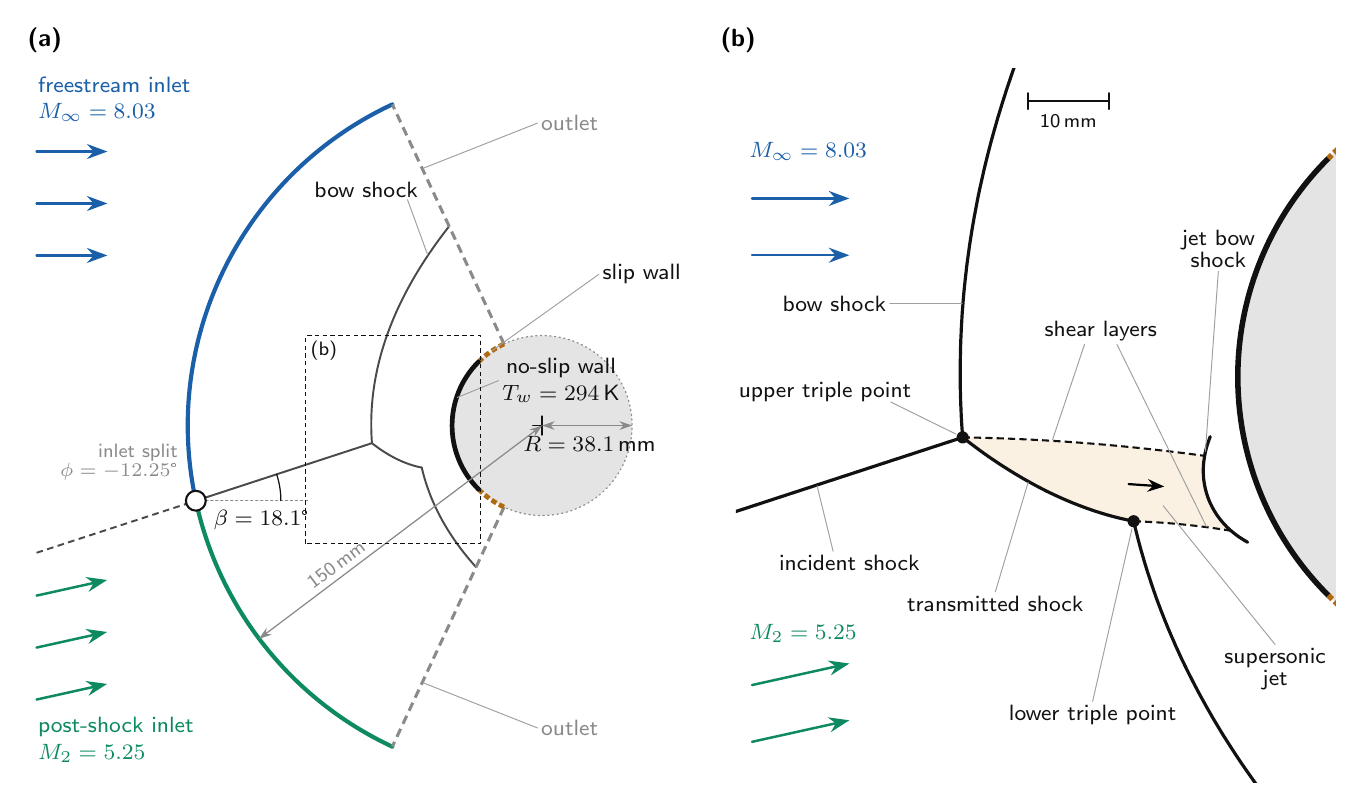
\begin{tikzpicture}[
    x=1mm, y=1mm,
    line cap=round, line join=round,
    % --- labels and leaders
    lbl/.style={font=\sffamily\footnotesize, text=ink, inner sep=1.2pt, align=center},
    small/.style={font=\sffamily\scriptsize},
    leader/.style={draw=leadergrey, line width=0.35pt, shorten >=0.3pt},
    % --- domain boundaries
    freeinlet/.style={draw=freeblue, line width=1.5pt},
    postinlet/.style={draw=postgreen, line width=1.5pt},
    outlet/.style={draw=dimgrey, line width=1.1pt, dash pattern=on 3.2pt off 2pt, line cap=butt},
    noslip/.style={draw=ink, line width=1.7pt},
    slip/.style={draw=slipochre, line width=1.7pt, dash pattern=on 2pt off 1.1pt, line cap=butt},
    % --- flow features
    shockA/.style={draw=shockgrey, line width=0.7pt},
    shockB/.style={draw=ink, line width=1.15pt},
    shear/.style={draw=ink, line width=0.75pt, dash pattern=on 2.6pt off 1.5pt, line cap=butt},
    flow/.style={line width=0.9pt, -{Stealth[length=2.6mm, width=1.9mm]}},
    dim/.style={draw=dimgrey, line width=0.45pt, {Stealth[length=1.6mm, width=1.1mm]}-{Stealth[length=1.6mm, width=1.1mm]}},
    triple/.style={circle, fill=ink, inner sep=0pt, minimum size=1.55mm},
]

% ==========================================================================
%  (a)  computational domain        scale 1 : 3.333
% ==========================================================================
\begin{scope}[shift={(65.4,45.6)}, x=0.3mm, y=0.3mm]

  % cylinder (grey disk; dotted outline where it lies outside the domain)
  \fill[bodygrey] (0,0) circle[radius=38.1];
  \draw[dimgrey, line width=0.45pt, dash pattern=on 0.4pt off 1.3pt]
    (115.0:38.1) arc[start angle=115.0, end angle=-115.0, radius=38.1];

  % shock system (no-field solution), clipped to the domain
  \begin{scope}
    \clip (115.0:150.0) arc[start angle=115.0, end angle=245.0, radius=150.0]
          -- (245.0:38.1) arc[start angle=245.0, end angle=115.0, radius=38.1] -- cycle;
    % upper bow shock
    \draw[shockA]
      (-72.03,-7.46) -- (-72.18,-5.05) -- (-72.28,-2.64) -- (-72.33,-0.23) -- (-72.32,2.18) -- 
      (-72.25,4.59) -- (-72.13,7) -- (-71.96,9.41) -- (-71.73,11.82) -- (-71.45,14.23) -- 
      (-71.11,16.64) -- (-70.72,19.05) -- (-70.27,21.46) -- (-69.77,23.86) -- (-69.21,26.27) -- 
      (-68.6,28.68) -- (-67.94,31.09) -- (-67.22,33.5) -- (-66.44,35.91) -- (-65.62,38.32) -- 
      (-64.73,40.73) -- (-63.79,43.14) -- (-62.8,45.55) -- (-61.76,47.96) -- (-60.66,50.37) -- 
      (-59.5,52.78) -- (-58.29,55.19) -- (-57.03,57.6) -- (-55.71,60.01) -- (-54.34,62.42) -- 
      (-52.91,64.83) -- (-51.43,67.24) -- (-49.9,69.64) -- (-48.31,72.05) -- (-46.66,74.46) -- 
      (-44.97,76.87) -- (-43.22,79.28) -- (-41.41,81.69) -- (-39.55,84.1) -- (-37.64,86.51) -- 
      (-35.68,88.92) -- (-33.66,91.33) -- (-31.58,93.74) -- (-29.45,96.15) -- (-27.27,98.56) -- 
      (-25.04,100.97) -- (-22.75,103.38) -- (-20.41,105.79) -- (-18.02,108.2) -- 
      (-15.57,110.61) -- (-13.07,113.02) -- (-10.51,115.42) -- (-7.9,117.83) -- (-5.24,120.24) -- 
      (-2.53,122.65) -- (0.24,125.06) -- (3.06,127.47) -- (5.93,129.88) -- (8.86,132.29) -- 
      (11.83,134.7) -- (14.86,137.11) -- (17.95,139.52) -- (21.08,141.93) -- (24.27,144.34) -- 
      (27.51,146.75) -- (30.8,149.16) -- (34.15,151.57) -- (37.55,153.98) -- (41,156.39) -- 
      (44.5,158.8) -- (46.27,160);
    % lower bow shock
    \draw[shockA]
      (-50.94,-17.8) -- (-50.38,-20.09) -- (-49.75,-22.36) -- (-49.05,-24.62) -- 
      (-48.29,-26.86) -- (-47.46,-29.09) -- (-46.57,-31.3) -- (-45.61,-33.5) -- 
      (-44.58,-35.68) -- (-43.49,-37.85) -- (-42.34,-40.01) -- (-41.12,-42.15) -- 
      (-39.83,-44.28) -- (-38.48,-46.39) -- (-37.06,-48.49) -- (-35.58,-50.57) -- 
      (-34.04,-52.64) -- (-32.42,-54.7) -- (-30.75,-56.74) -- (-29.01,-58.76) -- 
      (-27.2,-60.77) -- (-25.33,-62.77) -- (-23.4,-64.75) -- (-21.4,-66.72) -- (-19.34,-68.68) -- 
      (-17.21,-70.62) -- (-15.02,-72.55) -- (-12.77,-74.46) -- (-10.45,-76.36) -- 
      (-8.07,-78.24) -- (-5.63,-80.11) -- (-3.12,-81.97) -- (-0.55,-83.81) -- (2.08,-85.64) -- 
      (4.77,-87.45) -- (7.53,-89.25) -- (10.35,-91.04) -- (13.23,-92.82) -- (16.17,-94.58) -- 
      (19.17,-96.32) -- (22.24,-98.05) -- (25.36,-99.77) -- (28.55,-101.48) -- (31.8,-103.17) -- 
      (35.1,-104.85) -- (38.47,-106.52) -- (41.9,-108.17) -- (45.38,-109.81) -- 
      (48.93,-111.43) -- (52.54,-113.05) -- (56.2,-114.65) -- (59.92,-116.23) -- 
      (63.71,-117.81) -- (67.55,-119.37) -- (71.44,-120.92) -- (75.4,-122.45) -- 
      (79.41,-123.97) -- (83.48,-125.48) -- (87.61,-126.98) -- (91.79,-128.47) -- 
      (96.03,-129.94) -- (100.33,-131.4) -- (104.68,-132.85) -- (109.09,-134.28) -- 
      (113.55,-135.71) -- (118.06,-137.12) -- (122.64,-138.52) -- (127.26,-139.9) -- 
      (131.94,-141.28) -- (136.67,-142.64) -- (139.06,-143.32);
    % transmitted shock
    \draw[shockA]
      (-72.03,-7.46) -- (-70.95,-8.29) -- (-69.87,-9.09) -- (-68.79,-9.86) -- (-67.7,-10.59) -- 
      (-66.62,-11.29) -- (-65.54,-11.96) -- (-64.46,-12.6) -- (-63.38,-13.2) -- (-62.3,-13.77) -- 
      (-61.22,-14.31) -- (-60.13,-14.82) -- (-59.05,-15.29) -- (-57.97,-15.73) -- 
      (-56.89,-16.14) -- (-55.81,-16.52) -- (-54.73,-16.86) -- (-53.65,-17.17) -- 
      (-52.56,-17.45) -- (-51.48,-17.69) -- (-50.94,-17.8);
    % incident (imposed oblique) shock inside the domain
    \draw[shockA] (-146.58,-31.83) -- (-72.03,-7.46);
  \end{scope}

  % imposed oblique shock upstream of the inlet
  \draw[shockA, dash pattern=on 2.4pt off 1.6pt, line cap=butt] (-214,-53.86) -- (-146.58,-31.83);

  % inlets
  \draw[freeinlet] (192.25:150.0) arc[start angle=192.25, end angle=115.0, radius=150.0];
  \draw[postinlet] (245.0:150.0) arc[start angle=245.0, end angle=192.25, radius=150.0];

  % outlets
  \draw[outlet] (115.0:38.1) -- (115.0:150.0);
  \draw[outlet] (245.0:38.1) -- (245.0:150.0);

  % walls: no-slip |phi| <= 45 deg, slip 45 < |phi| <= 65 deg
  \draw[slip]   (115.0:38.1) arc[start angle=115.0, end angle=135.0, radius=38.1];
  \draw[slip]   (225.0:38.1) arc[start angle=225.0, end angle=245.0, radius=38.1];
  \draw[noslip] (135.0:38.1) arc[start angle=135.0, end angle=225.0, radius=38.1];

  % cylinder centre
  \draw[ink, line width=0.5pt] (-4,0) -- (4,0) (0,-4) -- (0,4);

  % inlet split and shock angle beta
  \draw[dimgrey, line width=0.4pt, dash pattern=on 0.8pt off 1pt] (-146.58,-31.83) -- ++(48,0);
  \draw[ink, line width=0.45pt] (-146.58,-31.83) ++(36,0) arc[start angle=0, end angle=18.100000000000005, radius=36];
  \node[lbl, anchor=north west] at (-140.58,-34.33) {$\beta = 18.1$\textdegree};
  \filldraw[fill=white, draw=ink, line width=0.75pt] (-146.58,-31.83) circle[radius=4.2];
  \node[lbl, small, text=dimgrey, anchor=south east, align=right] at (-152.58,-24.83)
    {inlet split\\[-0.3ex]$\phi = -12.25$\textdegree};

  % inflow
  \foreach \yy in {116, 94, 72} {\draw[flow, freeblue] (-214,\yy) -- ++(30,0);}
  \foreach \yy in {-72, -94, -116} {\draw[flow, postgreen] (-214,\yy) -- ++(12.49:30.6);}
  \node[lbl, text=freeblue, anchor=south west, align=left] at (-215,127)
    {freestream inlet\\$M_\infty = 8.03$};
  \node[lbl, text=postgreen, anchor=north west, align=left] at (-215,-122)
    {post-shock inlet\\$M_2 = 5.25$};

  % boundary labels
  \node[lbl, anchor=center] (ns) at (8,19) {no-slip wall\\$T_w = 294$\,K};
  \draw[leader] (ns.west) -- (-36.24,11.77);
  \node[lbl, anchor=west] (sw) at (24,64) {slip wall};
  \draw[leader] (sw.west) -- (-21.31,31.59);
  \node[lbl, text=dimgrey, anchor=west] (o1) at (-2,128) {outlet};
  \draw[leader] (o1.west) -- (115.0:120);
  \node[lbl, text=dimgrey, anchor=west] (o2) at (-2,-128) {outlet};
  \draw[leader] (o2.west) -- (245.0:120);
  \node[lbl, anchor=west] (bs) at (-98,100) {bow shock};
  \draw[leader] (bs.south east) ++(-6,0.5) -- (-48.34,72);

  % dimensions
  \draw[dim] (0,0) -- (0:38.1);
  \node[lbl, anchor=north] at (20.05,-3) {$R = 38.1$\,mm};
  \draw[dim] (0,0) -- (217.0:150.0);
  \node[lbl, small, text=dimgrey, rotate=37.00] at (-87.17,-58.8) {150\,mm};

  % zoom window shown in (b)
  \draw[ink, line width=0.4pt, dash pattern=on 1.6pt off 1.2pt, line cap=butt]
    (-100.0,-50.0) rectangle (-26.0,38.0);
  \node[lbl, small, anchor=north west, inner sep=1.5pt] at (-100.0,38.0) {(b)};
\end{scope}

% ==========================================================================
%  (b)  type IV interaction          scale 1.03 : 1
% ==========================================================================
\begin{scope}[shift={(193,51.78)}, x=1.03mm, y=1.03mm]
  \begin{scope}
    \clip (-100.0,-50.0) rectangle (-26.0,38.0);

    % body and wall
    \fill[bodygrey] (0,0) circle[radius=38.1];
    \draw[noslip, line width=2pt] (135.0:38.1) arc[start angle=135.0, end angle=225.0, radius=38.1];
    \draw[slip, line width=2pt] (115.0:38.1) arc[start angle=115.0, end angle=135.0, radius=38.1];
    \draw[slip, line width=2pt] (225.0:38.1) arc[start angle=225.0, end angle=245.0, radius=38.1];

    % supersonic jet (light fill between the shear layers)
    \fill[jetfill]
      (-72.03,-7.46) .. controls (-62.08,-7.62) and (-52.14,-8.38) .. (-42.19,-9.74)
      -- (-42.19,-9.74) -- (-42.25,-10.1) -- (-42.3,-10.46) -- (-42.33,-10.82) -- (-42.35,-11.18) -- 
      (-42.36,-11.54) -- (-42.35,-11.9) -- (-42.33,-12.25) -- (-42.3,-12.6) -- (-42.26,-12.95) -- 
      (-42.21,-13.29) -- (-42.14,-13.64) -- (-42.06,-13.97) -- (-41.97,-14.31) -- 
      (-41.86,-14.64) -- (-41.75,-14.97) -- (-41.62,-15.29) -- (-41.48,-15.61) -- 
      (-41.33,-15.92) -- (-41.17,-16.23) -- (-40.99,-16.53) -- (-40.81,-16.83) -- 
      (-40.61,-17.12) -- (-40.4,-17.41) -- (-40.18,-17.69) -- (-39.95,-17.96) -- 
      (-39.71,-18.23) -- (-39.46,-18.49) -- (-39.19,-18.74) -- (-38.92,-18.98)
      .. controls (-42.93,-18.32) and (-46.94,-17.93) .. (-50.94,-17.8)
      -- (-50.94,-17.8) -- (-52.02,-17.57) -- (-53.11,-17.31) -- (-54.19,-17.02) -- 
      (-55.27,-16.69) -- (-56.35,-16.33) -- (-57.43,-15.94) -- (-58.51,-15.52) -- 
      (-59.59,-15.06) -- (-60.67,-14.57) -- (-61.76,-14.05) -- (-62.84,-13.49) -- 
      (-63.92,-12.9) -- (-65,-12.28) -- (-66.08,-11.63) -- (-67.16,-10.95) -- (-68.24,-10.23) -- 
      (-69.33,-9.48) -- (-70.41,-8.69) -- (-71.49,-7.88) -- (-72.03,-7.46) -- cycle;

    % upper bow shock
    \draw[shockB]
      (-72.03,-7.46) -- (-72.07,-6.88) -- (-72.11,-6.3) -- (-72.15,-5.72) -- (-72.18,-5.15) -- 
      (-72.21,-4.57) -- (-72.23,-3.99) -- (-72.26,-3.41) -- (-72.28,-2.83) -- (-72.29,-2.25) -- 
      (-72.31,-1.68) -- (-72.32,-1.1) -- (-72.32,-0.52) -- (-72.33,0.06) -- (-72.33,0.64) -- 
      (-72.33,1.21) -- (-72.32,1.79) -- (-72.31,2.37) -- (-72.3,2.95) -- (-72.29,3.53) -- 
      (-72.27,4.11) -- (-72.25,4.68) -- (-72.22,5.26) -- (-72.2,5.84) -- (-72.17,6.42) -- 
      (-72.13,7) -- (-72.1,7.57) -- (-72.06,8.15) -- (-72.01,8.73) -- (-71.97,9.31) -- 
      (-71.92,9.89) -- (-71.87,10.47) -- (-71.81,11.04) -- (-71.75,11.62) -- (-71.69,12.2) -- 
      (-71.62,12.78) -- (-71.56,13.36) -- (-71.49,13.93) -- (-71.41,14.51) -- (-71.33,15.09) -- 
      (-71.25,15.67) -- (-71.17,16.25) -- (-71.08,16.83) -- (-70.99,17.4) -- (-70.9,17.98) -- 
      (-70.8,18.56) -- (-70.7,19.14) -- (-70.6,19.72) -- (-70.49,20.29) -- (-70.38,20.87) -- 
      (-70.27,21.45) -- (-70.16,22.03) -- (-70.04,22.61) -- (-69.92,23.19) -- (-69.79,23.76) -- 
      (-69.66,24.34) -- (-69.53,24.92) -- (-69.4,25.5) -- (-69.26,26.08) -- (-69.12,26.65) -- 
      (-68.98,27.23) -- (-68.83,27.81) -- (-68.68,28.39) -- (-68.53,28.97) -- (-68.37,29.55) -- 
      (-68.21,30.12) -- (-68.05,30.7) -- (-67.88,31.28) -- (-67.72,31.86) -- (-67.54,32.44) -- 
      (-67.37,33.01) -- (-67.19,33.59) -- (-67.01,34.17) -- (-66.82,34.75) -- (-66.64,35.33) -- 
      (-66.45,35.91) -- (-66.25,36.48) -- (-66.06,37.06) -- (-65.86,37.64) -- (-65.65,38.22) -- 
      (-65.45,38.8) -- (-65.24,39.37) -- (-65.02,39.95) -- (-64.81,40.53) -- (-64.59,41.11) -- 
      (-64.37,41.69) -- (-64.14,42.27) -- (-63.91,42.84) -- (-63.68,43.42) -- (-63.45,44);
    % lower bow shock
    \draw[shockB]
      (-50.94,-17.8) -- (-50.81,-18.36) -- (-50.67,-18.92) -- (-50.53,-19.48) -- 
      (-50.39,-20.04) -- (-50.24,-20.6) -- (-50.09,-21.16) -- (-49.93,-21.71) -- 
      (-49.77,-22.27) -- (-49.61,-22.82) -- (-49.44,-23.38) -- (-49.27,-23.93) -- 
      (-49.09,-24.48) -- (-48.91,-25.03) -- (-48.73,-25.58) -- (-48.54,-26.13) -- 
      (-48.35,-26.68) -- (-48.16,-27.23) -- (-47.96,-27.77) -- (-47.75,-28.32) -- 
      (-47.55,-28.86) -- (-47.33,-29.41) -- (-47.12,-29.95) -- (-46.9,-30.49) -- 
      (-46.68,-31.03) -- (-46.45,-31.57) -- (-46.22,-32.11) -- (-45.98,-32.65) -- 
      (-45.75,-33.19) -- (-45.5,-33.73) -- (-45.26,-34.26) -- (-45.01,-34.8) -- 
      (-44.75,-35.33) -- (-44.49,-35.87) -- (-44.23,-36.4) -- (-43.96,-36.93) -- 
      (-43.69,-37.46) -- (-43.42,-37.99) -- (-43.14,-38.52) -- (-42.86,-39.05) -- 
      (-42.57,-39.58) -- (-42.28,-40.1) -- (-41.99,-40.63) -- (-41.69,-41.15) -- 
      (-41.39,-41.68) -- (-41.09,-42.2) -- (-40.78,-42.72) -- (-40.46,-43.25) -- 
      (-40.15,-43.77) -- (-39.83,-44.29) -- (-39.5,-44.8) -- (-39.17,-45.32) -- 
      (-38.84,-45.84) -- (-38.5,-46.36) -- (-38.16,-46.87) -- (-37.82,-47.39) -- 
      (-37.47,-47.9) -- (-37.12,-48.41) -- (-36.76,-48.92) -- (-36.4,-49.43) -- 
      (-36.04,-49.94) -- (-35.67,-50.45) -- (-35.3,-50.96) -- (-34.92,-51.47) -- 
      (-34.54,-51.98) -- (-34.16,-52.48) -- (-33.77,-52.99) -- (-33.38,-53.49) -- 
      (-32.98,-53.99) -- (-32.58,-54.5) -- (-32.18,-55) -- (-31.77,-55.5) -- (-31.36,-56);
    % incident shock
    \draw[shockB] (-104,-17.91) -- (-72.03,-7.46);
  \end{scope}

  % transmitted shock
  \draw[shockB]
    (-72.03,-7.46) -- (-71.49,-7.88) -- (-70.95,-8.29) -- (-70.41,-8.69) -- (-69.87,-9.09) -- 
      (-69.33,-9.48) -- (-68.79,-9.86) -- (-68.24,-10.23) -- (-67.7,-10.59) -- (-67.16,-10.95) -- 
      (-66.62,-11.29) -- (-66.08,-11.63) -- (-65.54,-11.96) -- (-65,-12.28) -- (-64.46,-12.6) -- 
      (-63.92,-12.9) -- (-63.38,-13.2) -- (-62.84,-13.49) -- (-62.3,-13.77) -- (-61.76,-14.05) -- 
      (-61.22,-14.31) -- (-60.67,-14.57) -- (-60.13,-14.82) -- (-59.59,-15.06) -- 
      (-59.05,-15.29) -- (-58.51,-15.52) -- (-57.97,-15.73) -- (-57.43,-15.94) -- 
      (-56.89,-16.14) -- (-56.35,-16.33) -- (-55.81,-16.52) -- (-55.27,-16.69) -- 
      (-54.73,-16.86) -- (-54.19,-17.02) -- (-53.65,-17.17) -- (-53.11,-17.31) -- 
      (-52.56,-17.45) -- (-52.02,-17.57) -- (-51.48,-17.69) -- (-50.94,-17.8);

  % shear layers
  \draw[shear] (-72.03,-7.46) .. controls (-62.08,-7.62) and (-52.14,-8.38) .. (-42.19,-9.74);
  \draw[shear] (-50.94,-17.8) .. controls (-46.94,-17.93) and (-42.93,-18.32) .. (-38.92,-18.98);

  % jet bow shock
  \draw[shockB]
    (-36.89,-20.39) -- (-37.25,-20.18) -- (-37.59,-19.97) -- (-37.93,-19.75) -- 
      (-38.25,-19.52) -- (-38.56,-19.28) -- (-38.86,-19.04) -- (-39.15,-18.78) -- 
      (-39.43,-18.52) -- (-39.69,-18.24) -- (-39.95,-17.96) -- (-40.19,-17.68) -- 
      (-40.42,-17.38) -- (-40.64,-17.08) -- (-40.84,-16.77) -- (-41.03,-16.46) -- 
      (-41.21,-16.14) -- (-41.38,-15.81) -- (-41.54,-15.48) -- (-41.68,-15.15) -- 
      (-41.81,-14.8) -- (-41.92,-14.46) -- (-42.02,-14.11) -- (-42.11,-13.75) -- 
      (-42.19,-13.39) -- (-42.25,-13.03) -- (-42.3,-12.67) -- (-42.33,-12.3) -- 
      (-42.35,-11.93) -- (-42.36,-11.55) -- (-42.35,-11.18) -- (-42.33,-10.8) -- 
      (-42.29,-10.42) -- (-42.24,-10.04) -- (-42.18,-9.66) -- (-42.1,-9.28) -- (-42.01,-8.9) -- 
      (-41.9,-8.52) -- (-41.78,-8.14) -- (-41.65,-7.75) -- (-41.5,-7.37);

  % triple points
  \node[triple] (T1) at (-72.03,-7.46) {};
  \node[triple] (T2) at (-50.94,-17.8) {};

  % jet direction
  \draw[flow, line width=0.8pt, -{Stealth[length=2.1mm, width=1.6mm]}] (-51.56,-13.22) -- (-47.17,-13.52);

  % inflow
  \foreach \yy in {22, 15} {\draw[flow, freeblue] (-98,\yy) -- ++(12,0);}
  \node[lbl, text=freeblue, anchor=south west] at (-98.8,26.2) {$M_\infty = 8.03$};
  \foreach \yy in {-38, -45} {\draw[flow, postgreen] (-98,\yy) -- ++(12.49:12.3);}
  \node[lbl, text=postgreen, anchor=south west] at (-98.8,-33.2) {$M_2 = 5.25$};

  % labels
  \node[lbl, anchor=east] (lbow) at (-81,9) {bow shock};
  \draw[leader] (lbow.east) -- (-71.99,9);
  \node[lbl, anchor=south] (lt1) at (-89,-3.5) {upper triple point};
  \draw[leader] (lt1.south east) ++(-3,0.4) -- (T1);
  \node[lbl, anchor=north] (linc) at (-86,-21.5) {incident shock};
  \draw[leader] (linc.north) ++(-2,0) -- (-90,-13.33);
  \node[lbl, anchor=north] (ltr) at (-68,-26.5) {transmitted shock};
  \draw[leader] (ltr.north) -- (-63.92,-12.9);
  \node[lbl, anchor=north] (lt2) at (-56,-40) {lower triple point};
  \draw[leader] (lt2.north) -- (T2);
  \node[lbl, anchor=south] (lsl) at (-55,4) {shear layers};
  \draw[leader] (lsl.south) ++(-2,0) -- (-60.99,-7.88);
  \draw[leader] (lsl.south) ++(2,0) -- (-41.93,-18.54);
  \node[lbl, anchor=south] (ljs) at (-40.5,13) {jet bow\\[-0.4ex]shock};
  \draw[leader] (ljs.south) -- (-42.1,-9.28);
  \node[lbl, anchor=north] (ljet) at (-33.5,-33) {supersonic\\[-0.4ex]jet};
  \draw[leader] (ljet.north) -- (-47.36,-15.82);

  % scale bar
  \draw[ink, line width=0.8pt, line cap=butt] (-64,34) -- (-54,34);
  \draw[ink, line width=0.6pt] (-64,33) -- (-64,35) (-54,33) -- (-54,35);
  \node[lbl, small, anchor=north] at (-59,32.8) {10\,mm};
\end{scope}

% panel letters
\node[anchor=north west, inner sep=0pt, font=\sffamily\bfseries\small] at (0,96.2) {(a)};
\node[anchor=north west, inner sep=0pt, font=\sffamily\bfseries\small] at (88,96.2) {(b)};

\end{tikzpicture}
\end{document}
